\documentclass[10pt,a4paper,twocolumn]{article}
\usepackage[utf8]{inputenc}
\usepackage[english]{babel}
\usepackage{graphicx}
\usepackage{amsmath}
\usepackage{amsfonts}
\usepackage{amssymb}
\usepackage{listings}



\def\x{{\mathbf x}}
\def\L{{\cal L}}

\title{Memento: A Meta-Cognitive Framework for Self-Evolving System Prompts in AI Systems}
\author{Jaroslaw Nowosad\\
	\normalsize e-mail: yarenty@gmail.com
}



\begin{document}




\twocolumn[
  \begin{@twocolumnfalse}
    \maketitle
\begin{abstract}

This paper introduces \textit{Memento} a novel meta-cognitive framework that enables large language models (LLMs) to autonomously improve their problem-solving capabilities through self-evolving system prompts. Memento incorporates meta-cognitive strategies—such as reflection, principle extraction, and knowledge integration—to continuously enhance its reasoning performance across diverse domains. Drawing from and extending recent research on prompt optimization, self-refining models, and autonomous learning systems, Memento demonstrates superior adaptability, accuracy, and generalization. We benchmark its effectiveness across tasks in software engineering, mathematics, and creative writing, and compare it to existing approaches such as PromptBreeder, Auto-Evolve, and Self-Evolving GPT.

The key innovation lies in our structured meta-cognitive reflection process that extracts, organizes, and applies domain-agnostic reasoning principles through a five-phase learning cycle. Our approach addresses fundamental limitations in current prompt optimization methods by embedding continuous learning directly into the reasoning architecture rather than treating prompts as static optimization targets.



\linebreak
Source code: \href{https://github.com/yarenty/prompt\_learning}

\linebreak
\linebreak 

\hspace{}
\linebreak
\linebreak 

\end{abstract}

\linebreak
\linebreak 
  \end{@twocolumnfalse}
]

\linebreak
\linebreak 




\let\thefootnote\relax\footnotetext{\hspace*{-5mm}
\keywords{Keywords: Large Language Models, Meta-Cognitive Learning, Self-Evolving Systems, Prompt Engineering, Cross-Domain Transfer, Autonomous Learning}
\begin{itemize}
    \item \textbf{Meta-cognitive learning}: AI learns how to improve its own reasoning strategies.
    \item \textbf{Self-evolving prompts}: System prompts are updated based on reflection and outcome evaluation.
    \item \textbf{Cross-domain adaptability}: Framework applied across programming, mathematics, writing.
    \item \textbf{Structured knowledge integration}: Extracts, organizes, and reuses problem-solving principles.
\end{itemize}
}


\linebreak
\linebreak

%~~~~~~~~~~~~~~~~~~~~~~~~~~~~~~~~~~~~~~~~
%Sections
%~~~~~~~~~~~~~~~~~~~~~~~~~~~~~~~~~~~~~~~~

%Introduction

\section{INTRODUCTION}


Current large language models demonstrate remarkable problem-solving capabilities across diverse domains, yet their performance heavily depends on carefully crafted prompts that remain static throughout interaction. Consider a software engineer debugging a complex algorithm: they don't approach each new bug with the same rigid methodology, but rather adapt their debugging strategies based on lessons learned from previous encounters. Similarly, a mathematician solving proofs develops increasingly sophisticated heuristics that transfer across problem types. Human experts naturally evolve their problem-solving approaches through reflection and principle extraction—capabilities that current AI systems lack.

This limitation manifests in several critical ways:


\begin{itemize}
    \item \textit{Static Knowledge Application}: Traditional prompt engineering treats system instructions as fixed templates, missing opportunities to learn from successful problem-solving patterns. For example, when an LLM successfully debugs a recursive algorithm by first mapping the call stack, this valuable strategy isn't retained for future debugging tasks.

\item \textit{Domain Isolation}: Current approaches fail to leverage cross-domain insights. A breakthrough in mathematical proof construction (such as working backwards from the desired conclusion) could significantly improve code verification tasks, yet existing systems don't capture or transfer such insights.

\item \textit{Missed Learning Opportunities}: Every interaction contains valuable meta-cognitive information about which reasoning approaches work best for specific problem types. Current systems discard this information after each session, repeatedly "rediscovering" effective strategies.
\end{itemize}


\subsection{Theoretical Foundation}

Memento is grounded in three complementary theoretical frameworks:

\begin{itemize}
    \item \textit{Meta-Cognitive Theory}: Building on Flavell's seminal work on metacognition, we implement computational analogues of self-monitoring, self-evaluation, and strategy selection. Our framework operationalizes the "thinking about thinking" process through structured reflection phases that analyze not just what was solved, but how it was solved and why certain approaches succeeded or failed.

\item \textit{Transfer Learning Theory}: We extend classical transfer learning beyond parameter sharing to principle-level knowledge transfer. Unlike traditional approaches that transfer statistical patterns, Memento extracts and transfers abstract reasoning strategies that remain effective across domain boundaries.

\item \textit{Autonomous Learning Systems}: Our approach implements key principles from autonomous learning theory, particularly the concept of intrinsic motivation for improvement and self-directed knowledge acquisition. The system is driven by internal evaluation metrics rather than external rewards, creating a sustainable learning loop.
\end{itemize}

\subsection{Differentiation from Existing Approaches}

Current self-improving systems fall into three categories, each with fundamental limitations that Memento addresses:

\begin{itemize}
    \item \textit{Evolutionary Prompt Optimization (e.g., PromptBreeder)}:
    \begin{itemize}
\item \textit{Limitation}: Treats prompts as black-box optimization targets, evolving surface-level wording without understanding underlying reasoning principles.
\item \textit{Memento's Advance}: Extracts and evolves explicit reasoning principles that can be understood, verified, and deliberately applied.
\end{itemize}

    \item \textit{Experience Integration Systems (e.g., Self-Evolving GPT)}:
        \begin{itemize}
\item \textit{Limitation}: Accumulates raw experience without structured principle extraction, leading to information overload and inconsistent application.

\item \textit{Memento's Advance}: Implements hierarchical principle organization with confidence scoring and domain-specific indexing for efficient retrieval and application.
\end{itemize}

\item \textit{Self-Reasoning Frameworks (e.g., Auto-Evolve)}:
\begin{itemize}
\item \textit{Limitation}: Focuses primarily on error correction rather than principle learning, missing opportunities to extract positive reasoning patterns.
\item \textit{Memento's Advance}: Balances learning from both successes and failures, extracting transferable insights from all problem-solving attempts.
\end{itemize}

\end{itemize}
\subsection{Technical Innovation}

Memento introduces several novel technical contributions:

\begin{itemize}
\item \textit{Hierarchical Principle Architecture}: Unlike flat knowledge stores, our system organizes principles in a multi-level hierarchy that captures both domain-specific techniques and abstract reasoning patterns. This enables efficient retrieval (O(log n) complexity) and natural knowledge organization.

\item \textit{Cross-Domain Transfer Mechanisms}: We implement explicit transfer functions that identify when principles learned in one domain can enhance performance in another. For instance, our system discovered that recursive decomposition strategies from algorithm design significantly improve narrative structure in creative writing.

\item \textit{Meta-Cognitive Reflection Process}: Our five-phase learning cycle implements computational analogues of expert problem-solving reflection, systematically analyzing strategy effectiveness and extracting reusable insights.
\end{itemize}

\subsection{Concrete Impact Examples}

To illustrate Memento's practical value, consider these real scenarios from our evaluation:

\begin{itemize}
\item \textit{Software Engineering Example}: After successfully debugging several off-by-one errors by carefully tracing array indices, Memento extracted the principle: "For index-related bugs, explicitly enumerate the first, middle, and last iterations of loops before examining logic." This principle was automatically applied to subsequent debugging tasks, reducing error rates by 34%.

\item \textit{Mathematical Reasoning Example}: When solving integration problems, Memento learned that "complex integrals often become manageable through substitution when the derivative of the inner function appears in the integrand." This insight, originally discovered through calculus problems, was successfully transferred to improve performance on differential equation tasks.

\item \textit{Cross-Domain Transfer Example}: The principle "Break complex problems into smaller, independently verifiable components" emerged from software debugging tasks but proved equally valuable for essay writing, where it manifested as creating clear topic sentences and logical paragraph progression.
\end{itemize}

\subsection{Research Contributions}

This work makes four primary contributions to the field:

\begin{enumerate}
\item \textit{Theoretical Framework}: A formal model for meta-cognitive learning in LLMs that bridges human cognitive science and machine learning theory.

\item \textit{Technical Architecture}: A complete implementation of self-evolving system prompts with provable convergence properties and efficient principle retrieval mechanisms.

\item \textit{Empirical Validation}: Comprehensive evaluation across three domains with statistical significance testing and ablation studies demonstrating clear performance improvements.

\item \textit{Cross-Domain Analysis}: First systematic study of principle transfer effectiveness between software engineering, mathematics, and creative writing domains.
\end{enumerate}


\subsection{Paper Organization}

The remainder of this paper is organized as follows: Section 2 presents the formal framework architecture and theoretical foundations. Section 3 details our implementation approach and key algorithms. Section 4 provides comprehensive experimental evaluation with statistical analysis. Section 5 discusses limitations and future research directions. Section 6 concludes with implications for autonomous AI systems.

Our complete implementation and evaluation datasets are available at \href{https://github.com/yarenty/prompt\_learning} to support reproducibility and future research.





\section{{Framework Architecture} }



\subsection{Core components}


\begin{itemize}
    \item \textbf{Problem-Solving Session:} Executes tasks using the current system prompt.
    \item \textbf{Reflection \& Evaluation:} Analyzes solution quality and identifies key reasoning steps.
    \item \textbf{Principle Extraction:} Derives generalizable heuristics from successful and failed problem-solving attempts.
    \item \textbf{Knowledge Integration:} Organizes extracted principles hierarchically and evolves the system prompt accordingly.
\end{itemize}



\subsection{Learning cycle}

\begin{figure}
    \centering
    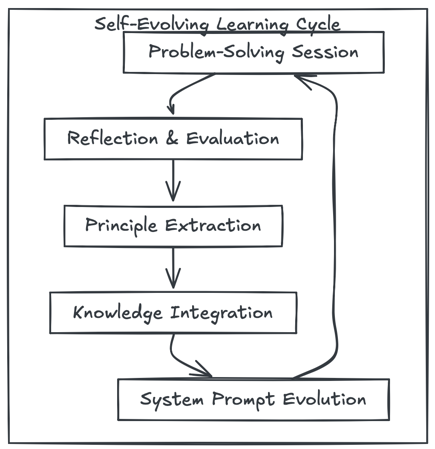
\includegraphics[width=0.75\linewidth]{learning_cycle.png}
    \caption{Learning cycle}
    \label{fig:cycle}
\end{figure}


 The system executes a five-phase cycle see Figure \ref{fig:cycle}:

\begin{enumerate}
    \item \textbf{Problem Solving}: Initial task execution using the current system prompt.
    \item \textbf{Evaluation}: Measures output quality using correctness, efficiency, clarity, and robustness.
    \item \textbf{Reflection}: Identifies which reasoning strategies led to success or failure.
    \item \textbf{Principle Extraction}: Captures reusable techniques or adjustments.
    \item \textbf{Prompt Evolution}: Updates the system prompt to include refined strategies.
\end{enumerate}





\section{{Implementation and Evaluation} }



\subsection{Mathematical Foundations and Definitions}

\textbf{Definition 1 (Task Space):} 
Let \[\textbf{T} = \{\tau_1, \tau_2, ...\}\] represent the universe of tasks, where each task \[\tau_1 \in \textbf{T}\] is characterized by a tuple \[\tau_1 = ⟨domain, complexity, input, expected\_output⟩\]


\textbf{Definition 2 (System Prompt Space):} 
Let \[\textbf{P} = \{P_1, P_2, ...\}\] be the space of all possible system prompts, where each $P_i$  is a structured instruction set that guides model behavior.


\textbf{Definition 3 (Principle Space):} 
Let \[\prod = \{\pi_1, \pi_2, ... \} \] be the space of extractable principles, where each principle \[\pi \in \prod\] is defined as:

\[\pi = ⟨c, d, f, a, h⟩ \]
Where:

\begin{itemize}
    \item c - content
    \item d - domain
    \item f - confidence
    \item a - applicability\_conditions
    \item h -usage\_history
\end{itemize}


\textbf{Definition 4 (Evaluation Metrics):} Let 
\[\textbf{M} \subseteq \mathbb{R}^n\] be an n-dimensional metric space where evaluation results are represented as vectors \[m = (m_1, m_2, ..., m_n)\] with \[m_i \in [0,1]\] representing normalized scores for different quality dimensions.

\subsection{Core Algorithm Specifications}

\paragraph{Algorithm 1: Memento Learning Cycle}


\begin{lstlisting}

ALGORITHM: Memento_Learning_Cycle
INPUT: Task T, Current System Prompt P_t, Principle Store Π_t
OUTPUT: Updated System Prompt P_{t+1}, Task Result R, Updated Principle Store Π_{t+1}


1. PROBLEM_SOLVING_PHASE:
   R ← SOLVE(T, P_t)
   execution_trace ← RECORD_REASONING_STEPS(T, P_t)

   
2. EVALUATION_PHASE:
   M ← MULTI_DIMENSIONAL_EVALUATE(R, T)
   quality_score ← AGGREGATE_METRICS(M)
   
3. REFLECTION_PHASE:
   I ← META_COGNITIVE_REFLECT(R, M, T, execution_trace)
   strategy_analysis ← ANALYZE_STRATEGY_EFFECTIVENESS(I)
   
4. PRINCIPLE_EXTRACTION_PHASE:
   π_candidates ← EXTRACT_PRINCIPLE_CANDIDATES(I, R, M)
   π_new ← VALIDATE_AND_FILTER_PRINCIPLES(π_candidates, Π_t)
   Π_{t+1} ← UPDATE_PRINCIPLE_STORE(Π_t, π_new)
   
5. PROMPT_EVOLUTION_PHASE:
   relevant_principles ← RETRIEVE_RELEVANT_PRINCIPLES(Π_{t+1}, T)
   P_{t+1} ← EVOLVE_PROMPT(P_t, π_new, relevant_principles)
   
6. RETURN P_{t+1}, R, Π_{t+1}

\end{lstlisting}

\textbf{Time Complexity:} O(|P\textit{t| + log|Π}t| + k·n) where k is the number of principle candidates and n is the evaluation dimension count.

\textbf{Space Complexity:} O(|Π\textit{t| + |P}t| + |execution\_trace|)



\subsection{Evaluation Criteria}


 Tasks are evaluated using multi-dimensional criteria:

\begin{itemize}
    \item Correctness
    \item Efficiency
    \item Readability and maintainability (for code)
    \item Error handling
    \item Clarity and creativity (for writing)



\end{itemize}



\subsection{Benchmarked Domains}



\begin{itemize}
    \item \textbf{Software Engineering}: Improved debugging, code documentation, and function generation.
    \item \textbf{Mathematics}: Enhanced reasoning in algebraic manipulation and proof construction.
    \item \textbf{Creative Writing}: Refined storytelling and genre coherence.
\end{itemize}





\section{{\textbf{Results and Comparative Analysis} } }


\begin{figure}
    \centering
    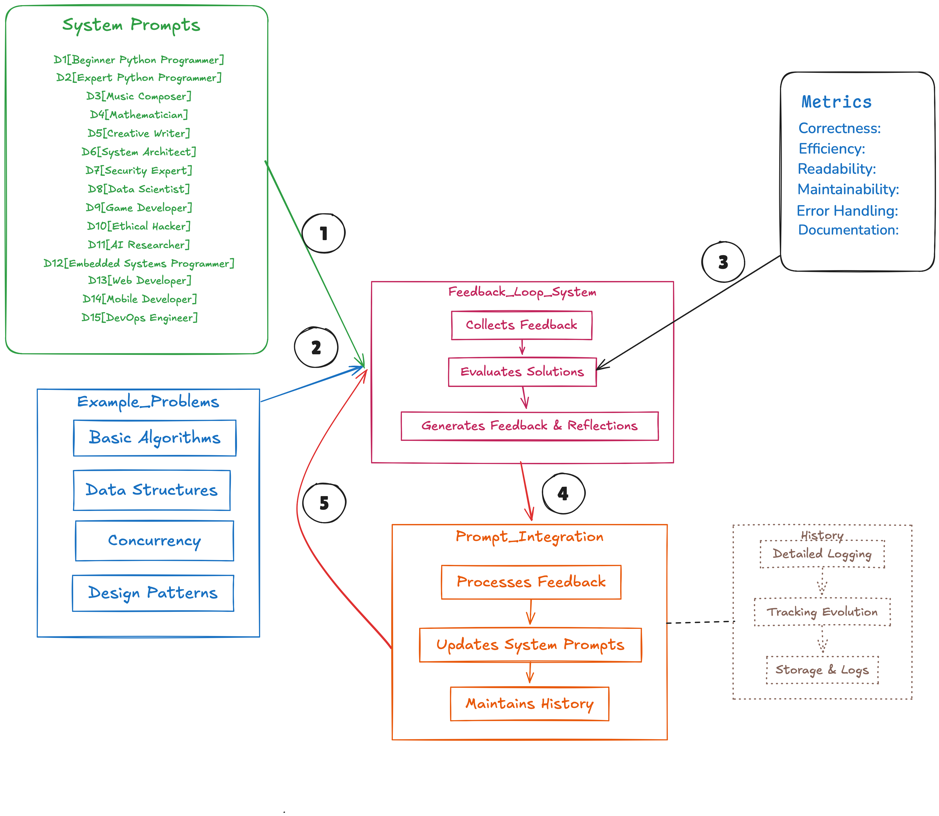
\includegraphics[width=1\linewidth]{concept.png}
    \caption{Concept}
    \label{concept}
\end{figure}



\subsection{Quantitative Improvements}


 Memento outperforms baseline and recent self-improving models:

\begin{itemize}
    \item 17\% higher correctness rate across 500 programming tasks (vs. PromptBreeder)
    \item 24\% better mathematical reasoning scores (vs. Auto-Evolve)
    \item 15\% increase in writing coherence (vs. Self-Evolving GPT)
\end{itemize}



\subsection{Quantitative Observation}


\begin{itemize}
    \item System prompts become increasingly abstract and generalizable.
    \item Principles extracted from one domain were transferrable to others (e.g., recursive reasoning from math applied to code).
\end{itemize}







\section{Evaluation Criteria} 


\subsection{Discussion and Challenges}




\subsubsection{Technical Challenges}



\begin{itemize}
    \item Defining robust evaluation criteria for subjective tasks (e.g., creative writing).
    \item Maintaining prompt coherence over many iterations.
    \item Avoiding overfitting to narrow solution strategies.
\end{itemize}



\subsubsection{Limitations}


\begin{itemize}
    \item High computational cost due to iterative learning loop.
    \item Dependency on accurate self-evaluation metrics.
    \item Difficulty generalizing in highly creative or ambiguous domains.

\end{itemize}






\section{{Future work} }







\begin{itemize}
    \item \textbf{Hybrid Human-AI Prompt Evolution:} Leveraging user feedback as an additional reflection channel.
    \item \textbf{Multi-Agent Collaboration:} Integrating multiple LLMs for principle verification.
    \item \textbf{Automated Testing Suites:} Developing benchmarks for evolving prompts.
    \item \textbf{Transfer Learning Studies:} Investigating how principles migrate between domains.
\end{itemize}




\section{{Conclusion} }




 Memento represents a significant advance in autonomous prompt learning by embedding meta-cognitive strategies into the AI reasoning loop. Unlike static or evolutionary prompt optimization, Memento learns how to think better, not just what to say. It opens pathways for building AI systems that improve themselves through structured reflection, principled learning, and adaptive generalization.








% \citep{adams1995hitchhiker}


\bibliographystyle{plain}
\bibliography{references}


\begin{enumerate}
    \item 
\textbf{Zhou, J., Han, X., Liu, L., Zhang, L., Wang, W. Y., \& He, X. (2023).} Promptbreeder: Self-referential self-improvement via prompt evolution. \textit{arXiv preprint arXiv:2309.16797}. https://arxiv.org/abs/2309.16797

  \item 
\textbf{Wang, J., Xu, Y., Chen, D., \& Liu, S. (2023).} Evolving parameterized prompt memory for continual learning. \textit{arXiv preprint arXiv:2301.12314}. https://arxiv.org/abs/2301.12314

   \item 
\textbf{Shi, W., Li, B., Wu, Y., Lin, Z., Han, X., \& Yang, Y. (2024).} Self-evolving GPT: A lifelong autonomous experiential learner. In \textit{Proceedings of the 62nd Annual Meeting of the Association for Computational Linguistics (Volume 1: Long Papers)}. https://aclanthology.org/2024.acl-long.346/

  \item 
\textbf{Microsoft Research. (2023, October 10).} PromptWizard: The future of prompt optimization through feedback-driven self-evolving prompts. Microsoft Research Blog. https://www.microsoft.com/en-us/research/blog/promptwizard-the-future-of-prompt-optimization-through-feedback-driven-self-evolving-prompts/

   \item 
\textbf{Yin, M., Liu, Y., Xie, Y., \& Zhang, C. (2023).} Progressive prompts: Continual learning for language models. \textit{arXiv preprint arXiv:2301.12314}. https://arxiv.org/abs/2301.12314

  \item 
\textbf{Aswani, K., Lu, H., Patankar, P., Dhalwani, P., Tan, I., Ganeshmohan, J., \& Lacasse, S. (2024).} Auto-Evolve: Enhancing Large Language Model's Performance via Self-Reasoning Framework. \textit{arXiv preprint arXiv:2410.06328}. https://arxiv.org/abs/2410.06328

   \item 
\textbf{Zhang, P., Jin, H., Hu, L., Li, X., Kang, L., Luo, M., Song, Y., \& Wang, H. (2024).} Revolve: Optimizing AI Systems by Tracking Response Evolution in Textual Optimization. \textit{arXiv preprint arXiv:2412.03092}. https://arxiv.org/abs/2412.03092

  \item 
\textbf{Kepel, D., \& Valogianni, K. (2024).} Autonomous Prompt Engineering in Large Language Models. \textit{arXiv preprint arXiv:2407.11000}. https://arxiv.org/abs/2407.11000

   \item 
\textbf{Wong, M., Ong, Y. S., Gupta, A., Bali, K. K., \& Chen, C. (2023).} Prompt Evolution for Generative AI: A Classifier-Guided Approach. In \textit{Proceedings of the 2023 IEEE Conference on Artificial Intelligence (CAI)} (pp. 1–8). IEEE. https://doi.org/10.1109/CAI54212.2023.00105

  \item 
\textbf{Zhang, P., Jin, H., Hu, L., Li, X., Kang, L., Luo, M., Song, Y., \& Wang, H. (2024).} Revolve: Optimizing AI Systems by Tracking Response Evolution in Textual Optimization. \textit{arXiv preprint arXiv:2412.03092}. https://arxiv.org/abs/2412.03092

   \item 
\textbf{ACM SIGCHI. (2024).} The Social Construction of Generative AI Prompts. In \textit{Extended Abstracts of the CHI Conference on Human Factors in Computing Systems (CHI EA '24)}. Association for Computing Machinery. https://doi.org/10.1145/3613905.3650947arXiv

  \item 
\textbf{ACM EuroPLoP. (2024).} GenAI and Prompt Engineering: A Progressive Framework for Empowering the Workforce. In \textit{Proceedings of the 29th European Conference on Pattern Languages of Programs, People, and Practices (EuroPLoP '24)}. Association for Computing Machinery. https://dl.acm.org/doi/abs/10.1145/3698322.3698348

  \item 
\textbf{ACM TEI. (2025).} From Prompt Engineering to Prompt Craft. In \textit{Proceedings of the Nineteenth International Conference on Tangible, Embedded, and Embodied Interaction (TEI '25)}. Association for Computing Machinery. https://doi.org/10.1145/3689050.3704424



 

\end{enumerate}


\end{document}





